\documentclass{article}

\usepackage[italian]{babel}
\usepackage[letterpaper,top=2cm,bottom=2cm,left=3cm,right=3cm,marginparwidth=1.75cm]{geometry}
\usepackage{amsmath}
\usepackage{graphicx}
\usepackage{subcaption}
\usepackage{textcomp}
\usepackage[colorlinks=true, allcolors=blue]{hyperref}
\usepackage{ragged2e}
\usepackage[dvipsnames]{xcolor}
\usepackage{fancyhdr}

\title{\textbf{Bivacco Casera Vignolet - 1340 m s.l.m}}
\author{Matteo Drago}

% ==========================================================
% Impostazioni per il logo in ogni pagina
% ==========================================================
\pagestyle{fancy}
\fancyhf{} % Pulisce tutti i campi di intestazione e piè di pagina
\fancyhead[R]{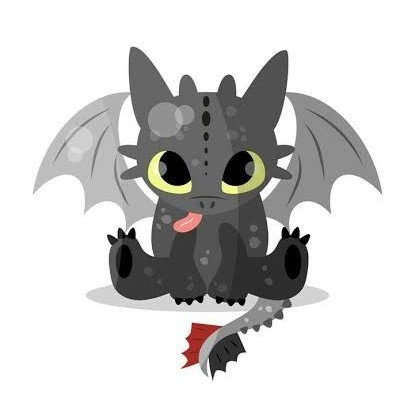
\includegraphics[height=1.5cm]{images/toothless.jpeg}} % Posiziona il logo a destra (R) nell'intestazione
\renewcommand{\headrulewidth}{0pt} % Rimuove la linea orizzontale nell'intestazione (opzionale)


\begin{document}
\maketitle
\thispagestyle{fancy} % Aggiungi questa riga

\begin{abstract}
Questo documento raccoglie e organizza le informazioni che ho acquisito nel corso degli anni sui bivacchi, basate sulle mie esperienze dirette. Sebbene non si proponga come una guida esaustiva e perfetta, offre il minimo indispensabile per una buona vita in bivacco, con consigli pratici e diretti per chiunque desideri affrontare al meglio queste pazze ma piacevoli avventure.
\end{abstract}

\section{Il bivacco}

% ==========================================================
% Immagine a sinistra, testo a destra allineato in alto
% ==========================================================
\noindent
\begin{minipage}[t]{0.45\textwidth}
  \vspace{0pt} % forza l'allineamento in alto
  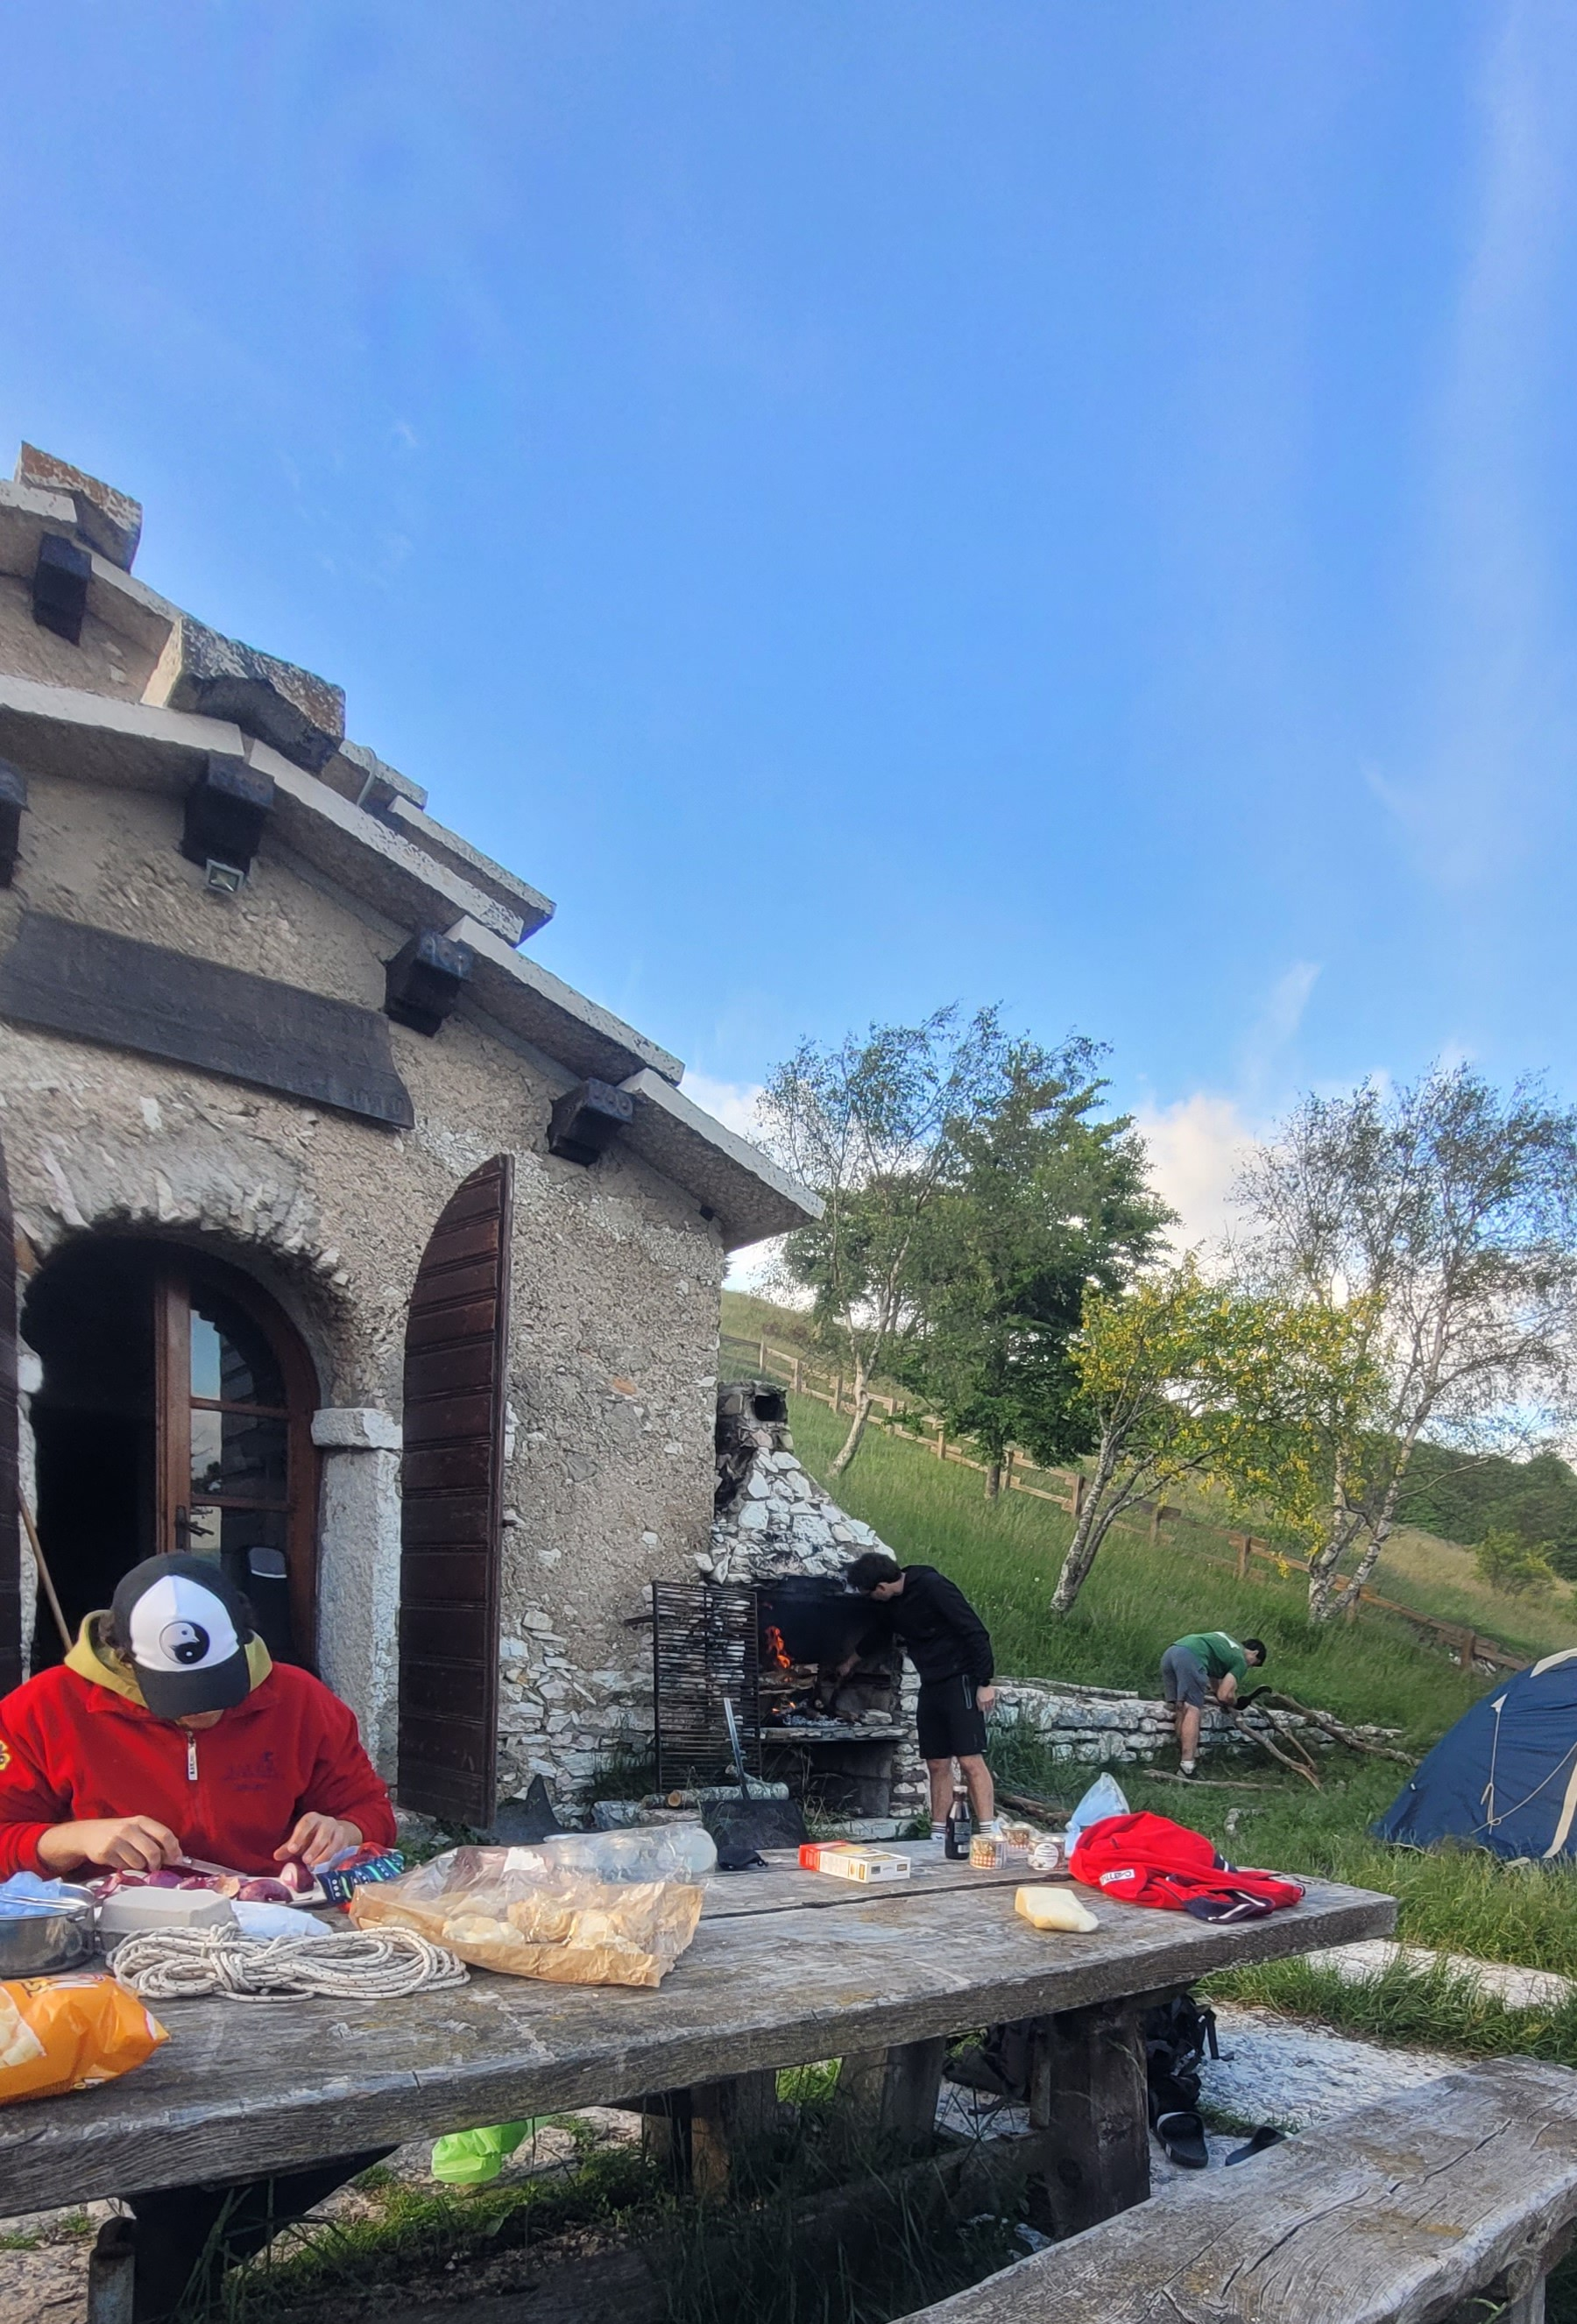
\includegraphics[width=\linewidth]{images/bivacco.jpg}
\end{minipage}%
\hfill
\begin{minipage}[t]{0.5\textwidth}
  \vspace{0pt} % forza l'allineamento in alto
  
  Gruppo montuoso\\
  \textbf{\large Monte Baldo}
  \\[1em] % Aggiunge una riga vuota qui
  Località\\
  \textbf{\large Monte Vignola – Prati di Vignoletto}
  \\[1em] % Aggiunge una riga vuota qui
  Comune\\  
  \textbf{\large Avio}
  \\[1em] % Aggiunge una riga vuota qui
  Altezza\\  
  \textbf{\large 1340 m s.l.m.}
  \\[1em] % Aggiunge una riga vuota qui
  Apertura\\  
  \textbf{\large Non gestito, sempre aperto}

\end{minipage}

\subsection{Caratteristiche}
Il bivacco Vignolet (ex-Casera Vignola) si trova a 1.340 metri sul versante meridionale del Monte Vignola, sull'altopiano di Brentonico

È circondato da un recinto e si presentano due edifici distinti.
\begin{itemize}
    \item \textbf{Primo edificio}: dormitorio, sono presenti sei posti letto su tre letti a castello. I materassi non ci sono.
    \item \textbf{Secondo edificio}: il corpo inferiore, si compone di un andito (con stufa a legna, cucina a gas e lavello con rubinetto) e di un altro locale, più interno, con tavolo, panche scavate nella pietra e caminetto, con funzione di saletta da pranzo (è anche presente un pannello solare sul tetto del bivacco che permette di avere un po' di luce all'interno dell'edificio.
    \item \textbf{Zona esterna}: si compone di un tavolo con panche, lavello in pietra con rubinetto e anche di un camino. L'acqua non è fornita durante l'inverno.
\end{itemize}

La presenza del lavello alleggerisce sicuramente il peso dello zaino. Non è molto piacevole dormire nello spazio adibito (un po' claustrofobico), proprio per questo motivo ci eravamo portati le tende.

Ricavare la legna è molto semplice data la presenza di un vasto bosco seguendo il sentiero che da sul bivacco. Il posto offre una vista spettacolare sulla valle dell'Adige (il bivacco si posiziona infatti in mezzo a un prato che strapiomba sulla valle dell'Adige, proprio sulla verticale del castello di Avio).

\section{Come ci siamo arrivati}
Abbiamo parcheggiato la macchina a Polsa di Monte Baldo arrivando verso le 11.00 del mattino e da li ci siamo incamminati. Pausa pranzo lungo il sentiero per poi arrivare al bivacco. Il giorno dopo abbiamo proseguito il nostro giro ad anello per tornare alla macchina.


\begin{figure}[htbp!]
    \centering
    % Colonna di sinistra, allineata in alto
    \begin{subfigure}[t]{0.45\textwidth}
        \centering
        \vspace{0pt} % Forziamo l'allineamento in alto
        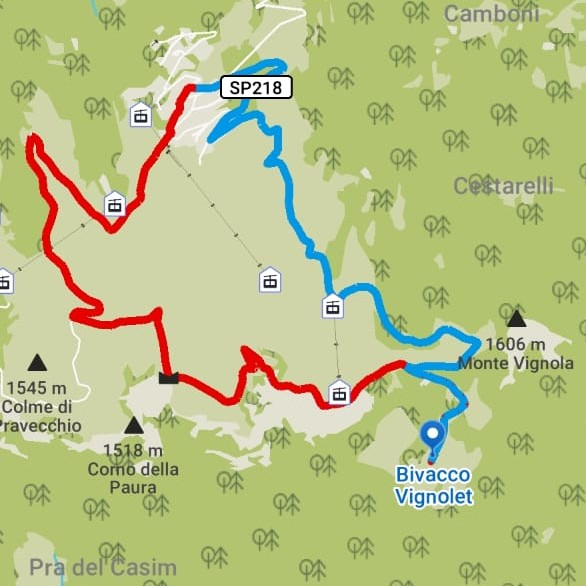
\includegraphics[width=\textwidth]{images/sentiero_mapsMe.jpg}
        \caption{Sentiero su Maps.Me.}
        \label{fig:foto_lunga}
    \end{subfigure}
    \hfill
    % Colonna di destra, allineata in alto
    \begin{subfigure}[t]{0.45\textwidth}
        \centering
        \vspace{0pt} % Forziamo l'allineamento in alto anche qui
        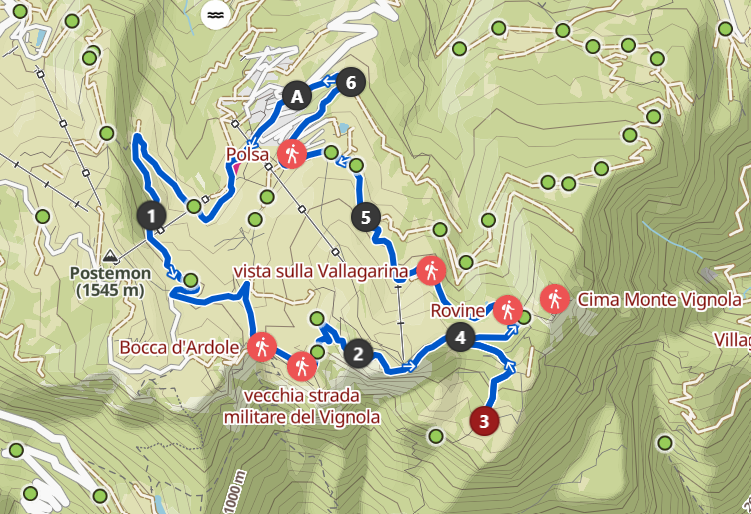
\includegraphics[width=\textwidth]{images/sentiero_komoot.png}
        \caption{Sentiero su Komoot.}
        \label{fig:foto_corta1}
        \vspace{1em} % Aggiunge un po' di spazio tra le due foto
        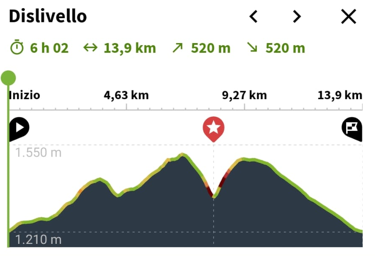
\includegraphics[width=\textwidth]{images/profilo_altimetrico.png}
        \caption{Profilo altimetrico del percorso.}
        \label{fig:foto_corta2}
    \end{subfigure}
    % Didascalia generale per l'intera figura
    \caption{Il sentiero e i dettagli del percorso.}
    \label{fig:panoramica_dettagli}
\end{figure}


\section{Non ti scordar di me}
\textbf{\textcolor{BurntOrange}{Ricorda: il bivacco è un bene comune. Il suo futuro dipende dal rispetto e dal senso civico dei visitatori. Usalo con cura e lascialo più pulito di come l'hai trovato.}}


\section{Alcune foto}

\begin{figure}[htbp!]
    \centering
    % Prima riga: Due foto affiancate
    \begin{subfigure}{0.45\textwidth}
        \centering
        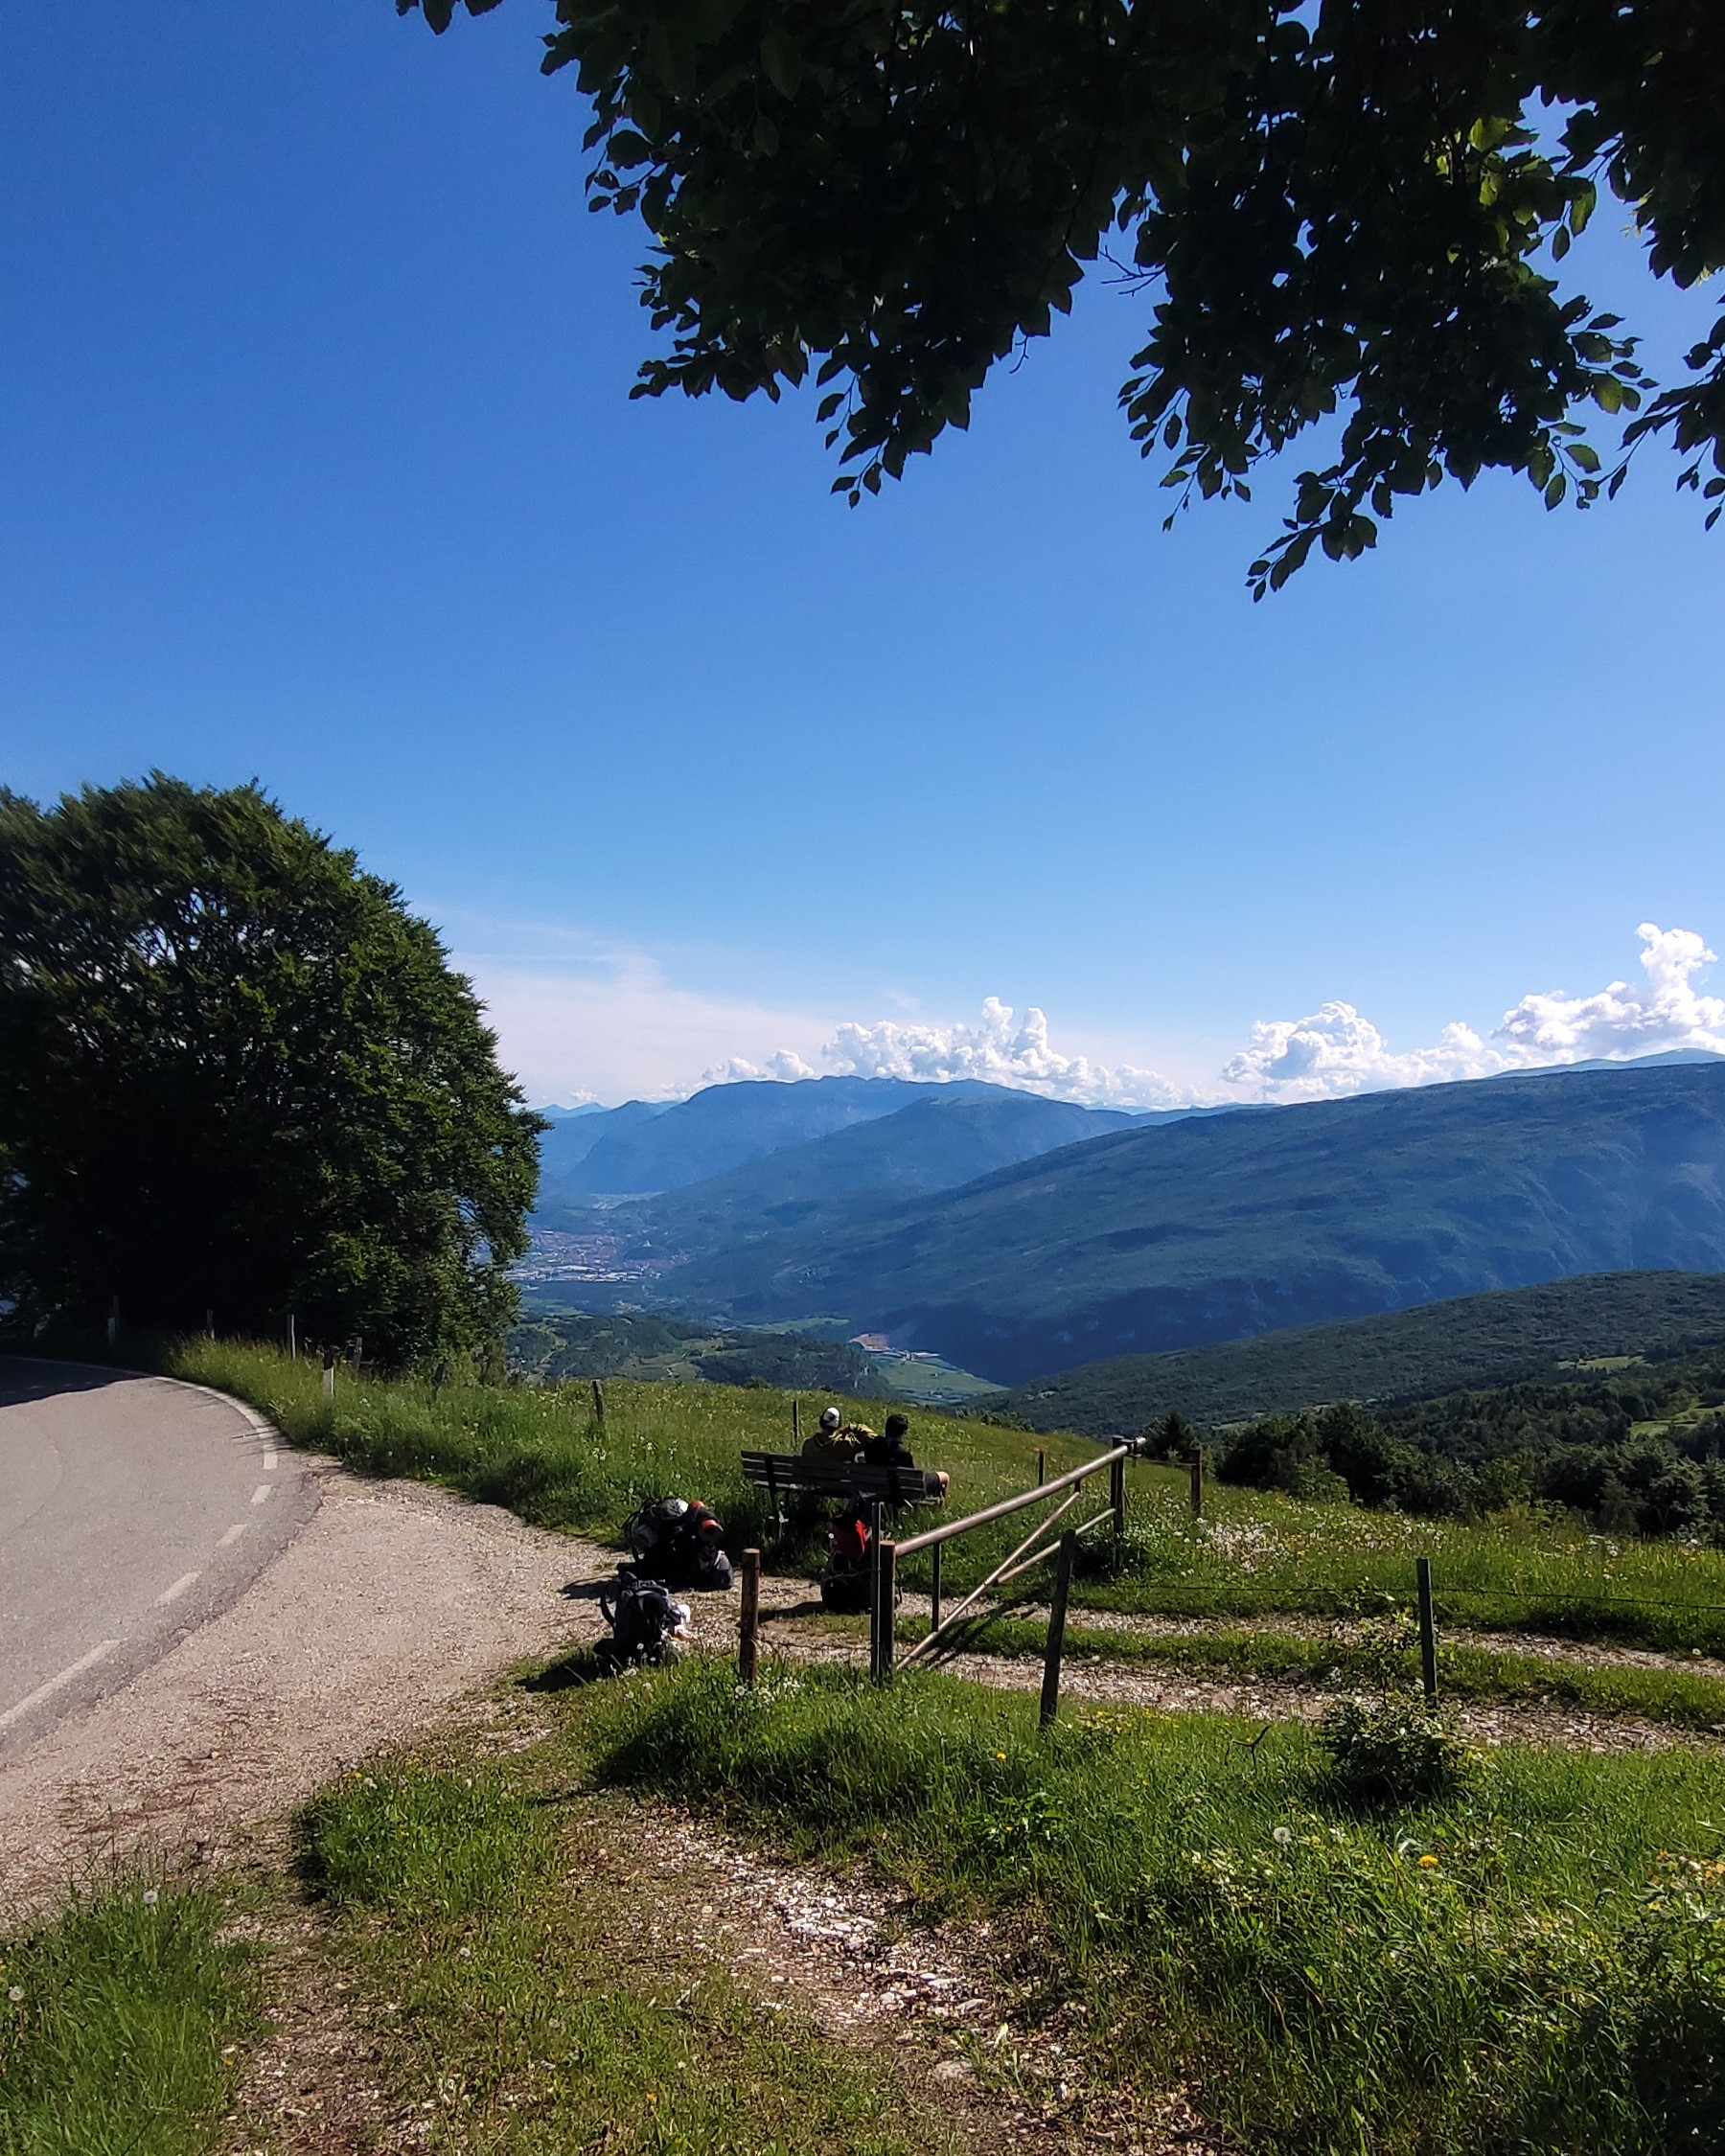
\includegraphics[width=\linewidth]{images/foto_panchina.jpg}
        \caption{Sentiero.}
        \label{fig:foto1}
    \end{subfigure}
    \hfill 
    \begin{subfigure}{0.45\textwidth}
        \centering
        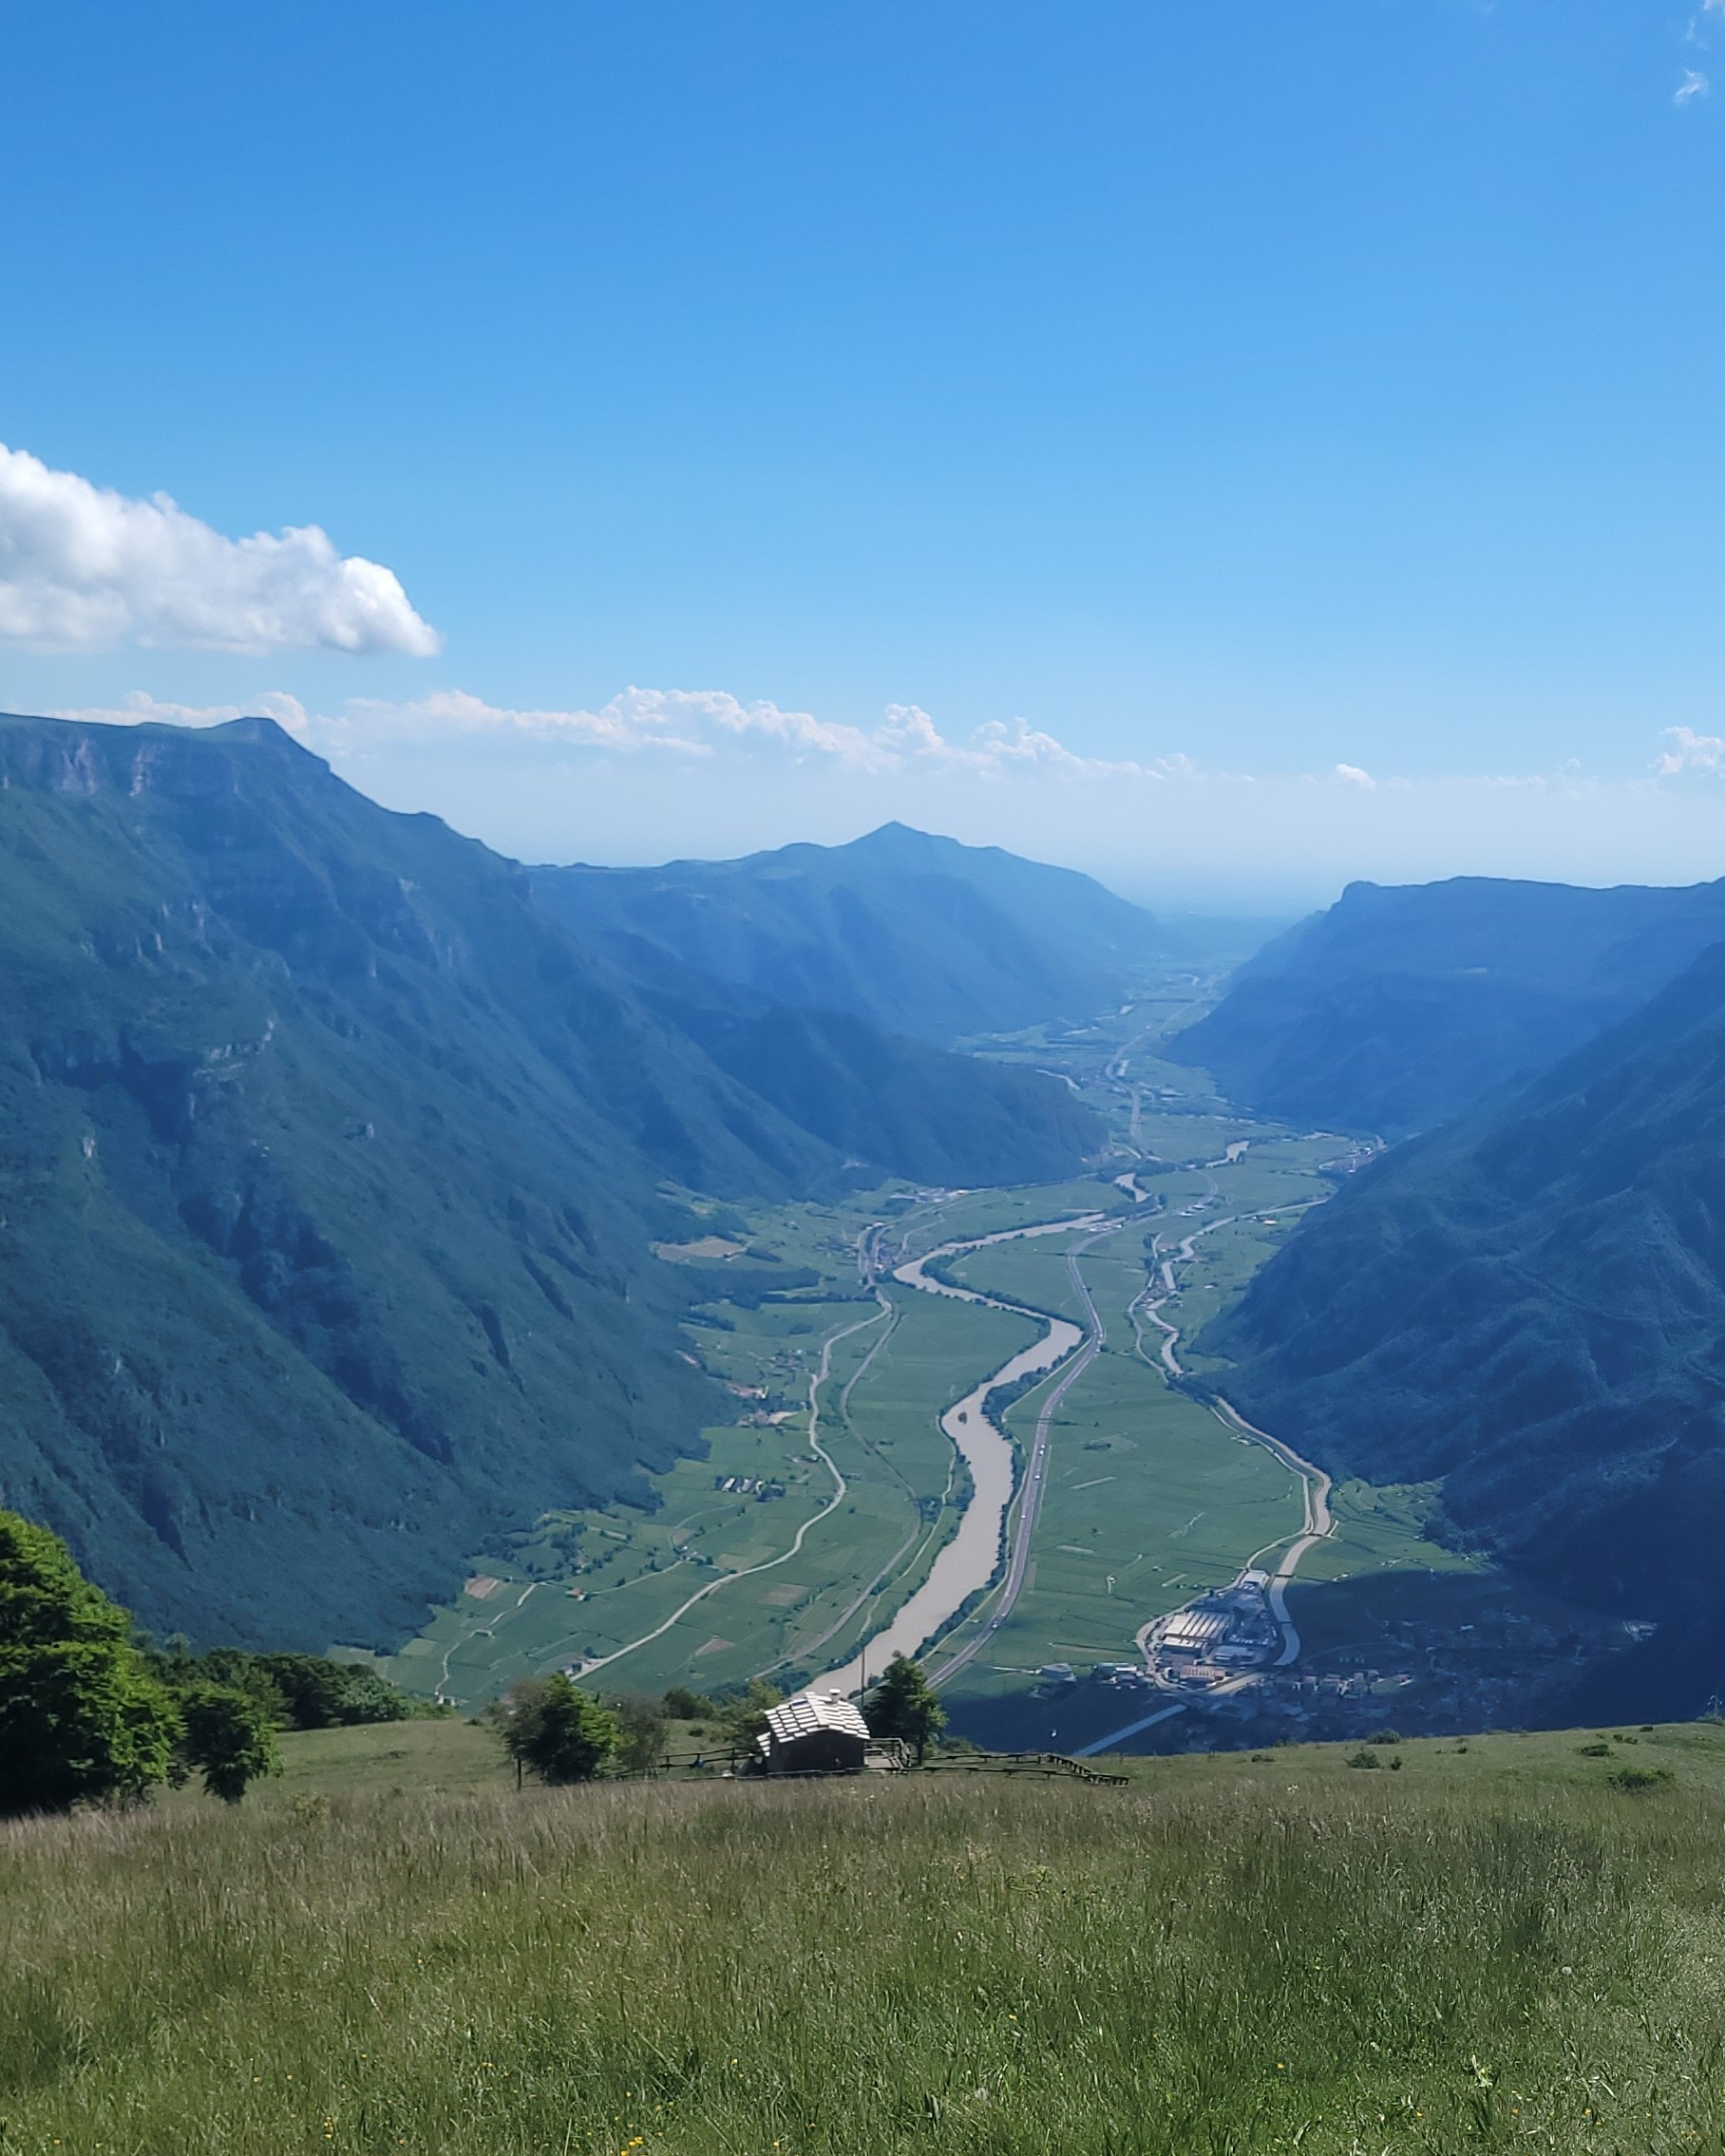
\includegraphics[width=\linewidth]{images/foto_bivaccoEvallata.jpg}
        \caption{Vista del bivacco e della vallata.}
        \label{fig:foto2}
    \end{subfigure}
    
    \vspace{2em} 
    
    % Seconda riga: Altre due foto affiancate
    \begin{subfigure}{0.45\textwidth}
        \centering
        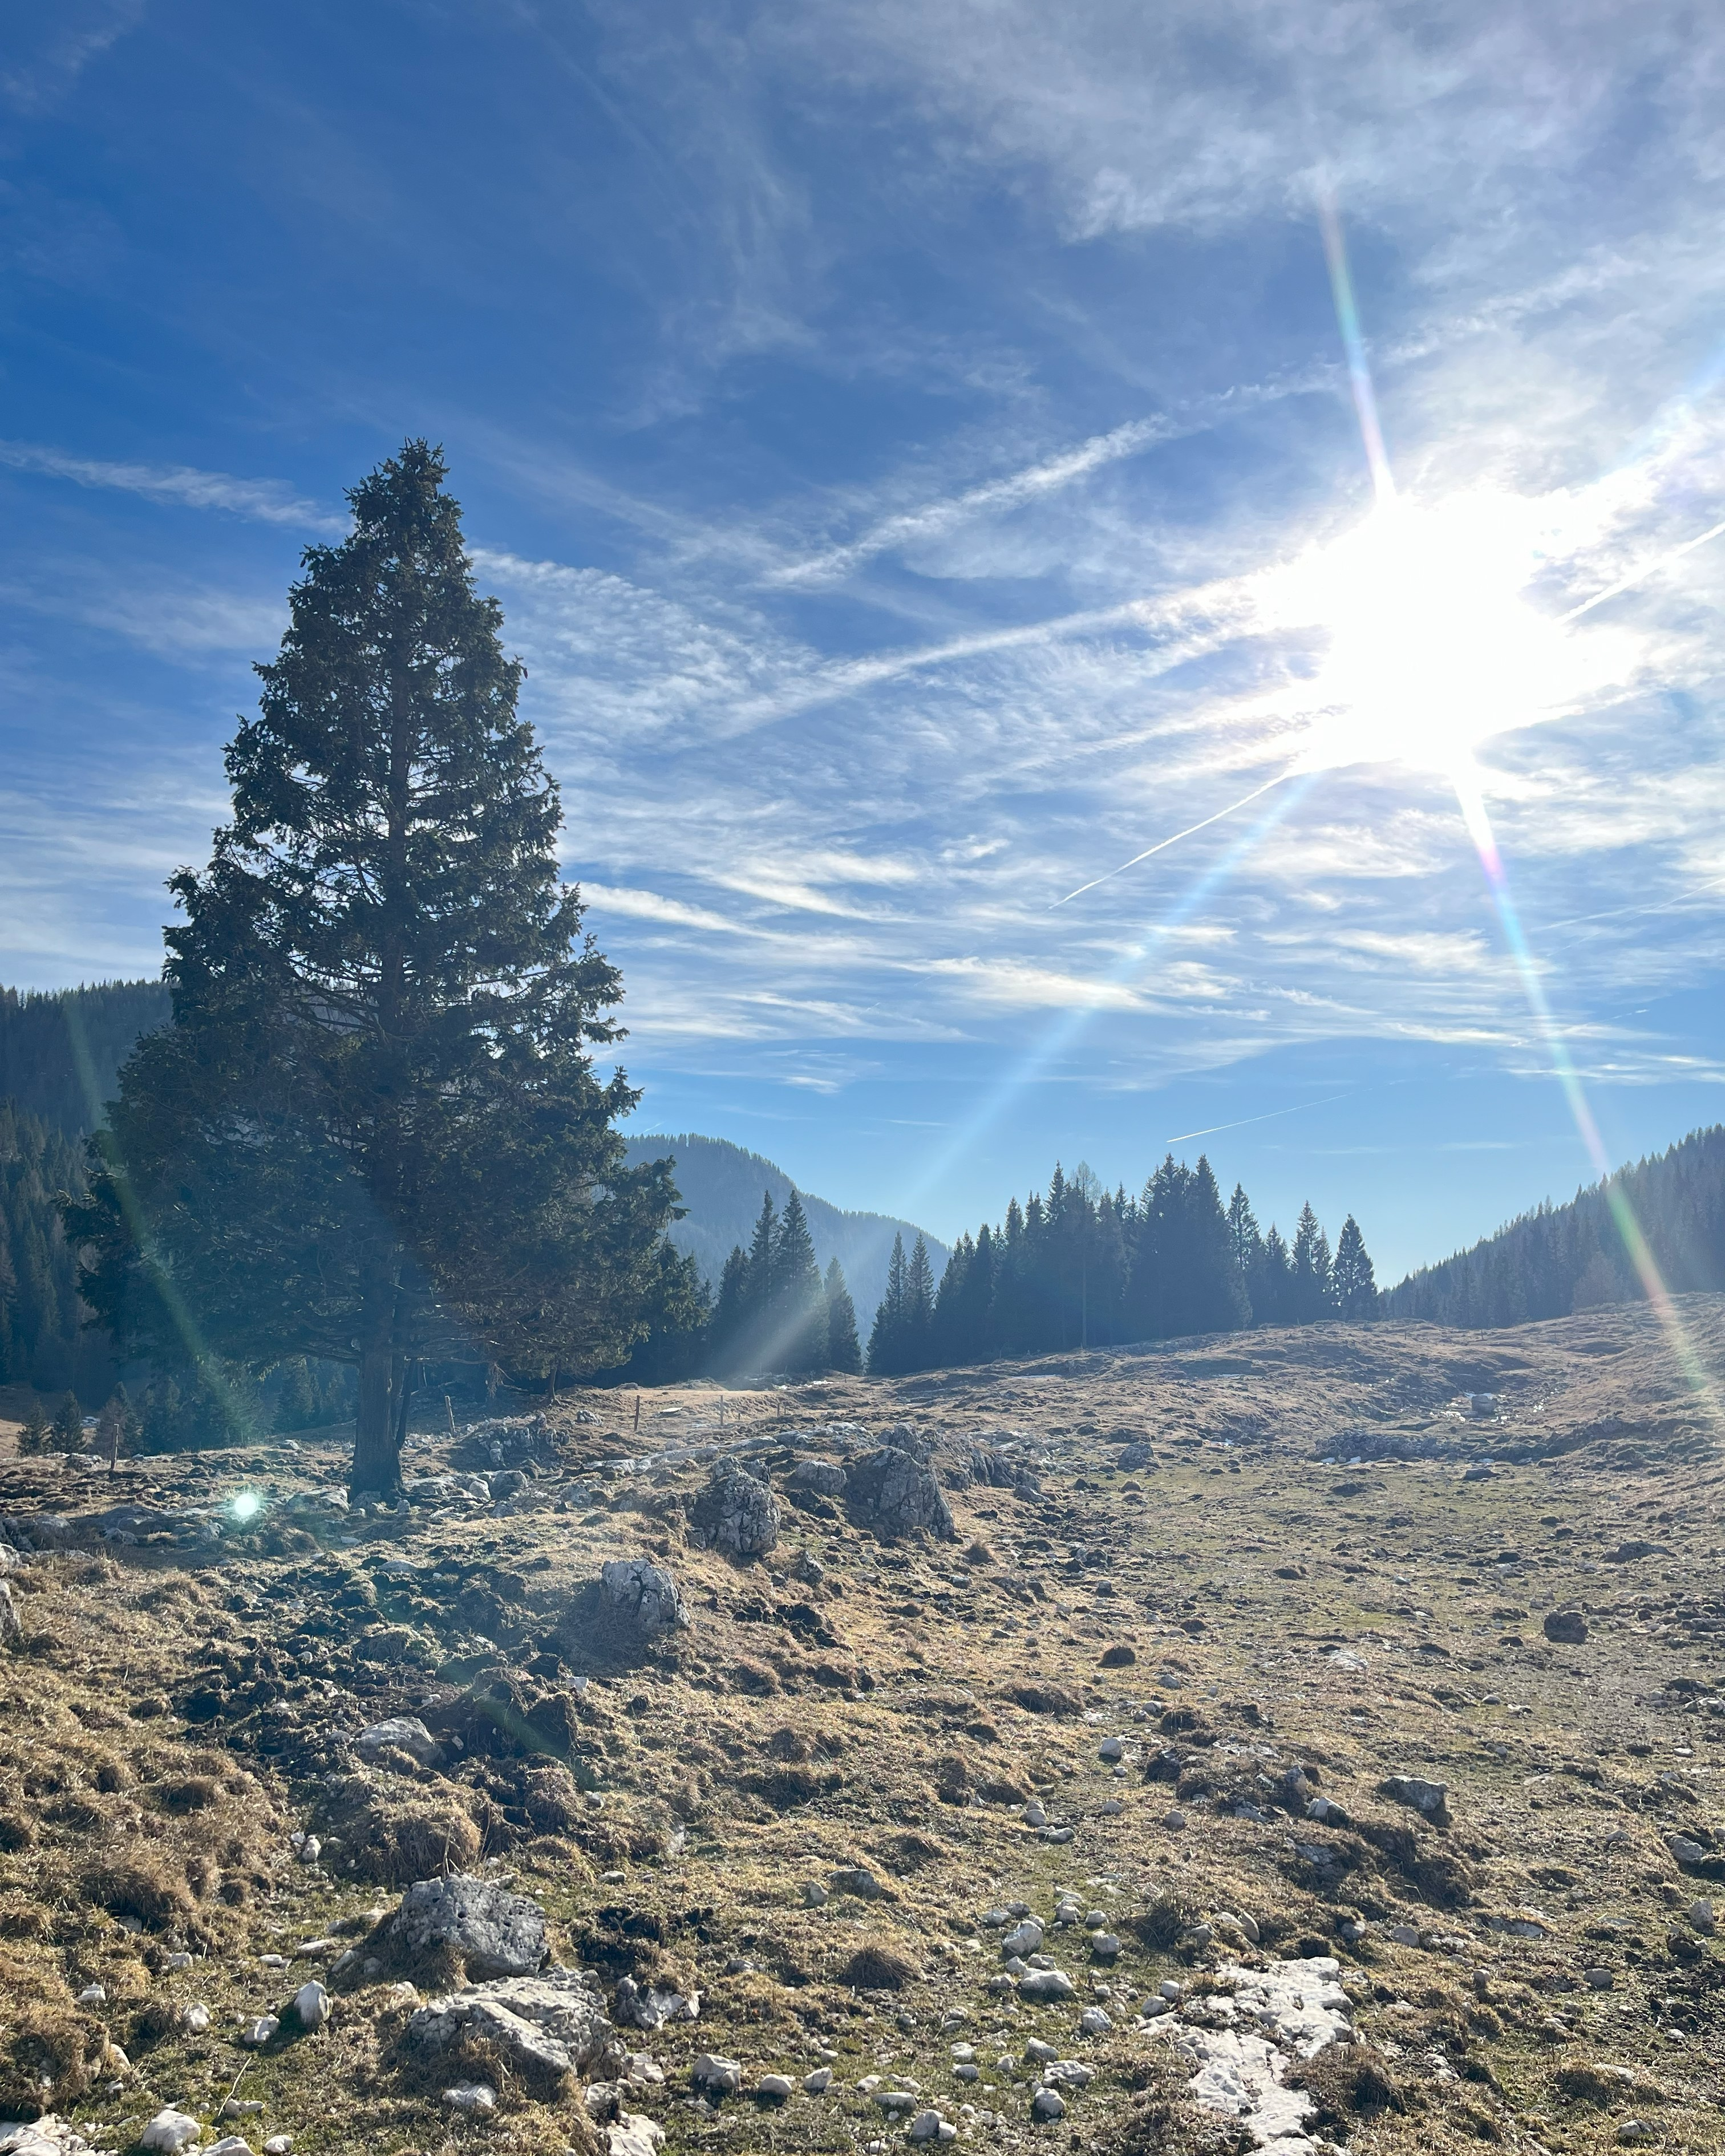
\includegraphics[width=\linewidth]{images/foto_paesaggio.jpg}
        \caption{Paesaggio.}
        \label{fig:foto3}
    \end{subfigure}
    \hfill 
    \begin{subfigure}{0.45\textwidth}
        \centering
        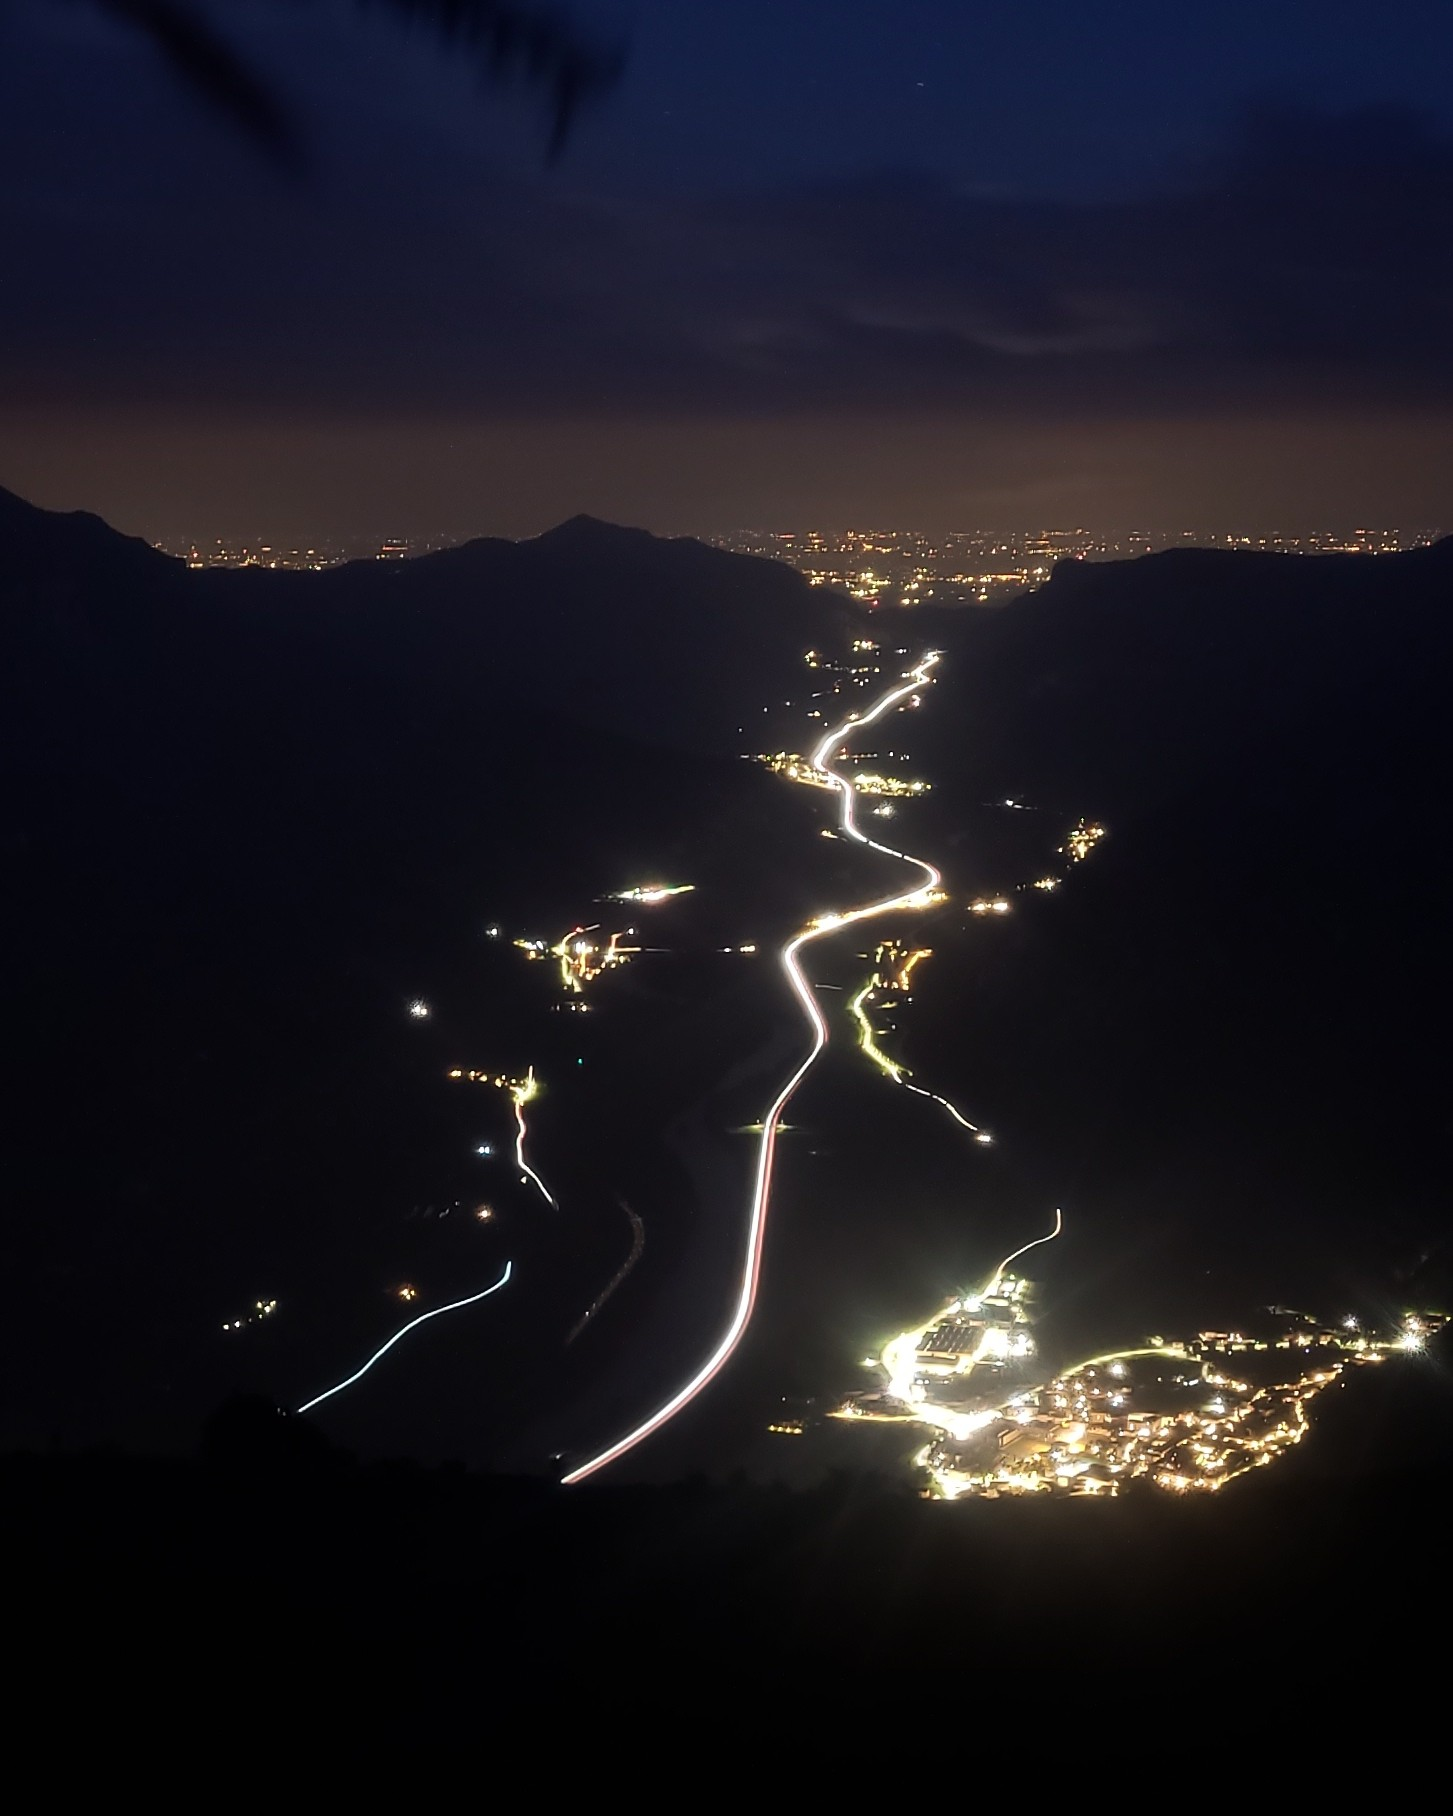
\includegraphics[width=\linewidth]{images/foto_vallataNotte.jpg}
        \caption{Vista della vallata di notte.}
        \label{fig:foto4}
    \end{subfigure}

    \caption{Selezione di fotografie del percorso e della vista dal bivacco.}
    \label{fig:panoramica_4_foto}
\end{figure}

\end{document}
